\chapter{Data Analysis and Modelling}
\label{chap:methods}




%%%%%%%%%%%%%%%%%%%%%%%%%%%%%
\draft{Why questionnaires and modelling?}

\section{Questionnaires}

 The full protocol developed for this thesis is outlined in \cref{chap:protocol}. The development and presentation of this protocol involved a substantial development and testing phase, and represents a novel advancement in soundscape survey methodology. Therefore it was submitted and published as a peer-reviewed journal article in MDPI Applied Sciences as \citet{Mitchell2020Soundscape} and is presented as a stand-alone chapter within this thesis. This section therefore presents those methods not associated with the data collection procedure, i.e. the analysis and statistical methods used.

\draft{from:} Published as: \textbf{Mitchell, A.}, Aletta, F., \& Kang, J. (2022). How to analyse and represent quantitative soundscape data. \emph{JASA Express Letters, 2}(13):037201.

\section*{Context}
The content of this chapter was originally published as \citet{Mitchell2022How}.

\section{Abstract}
This study first examines the methods presented in ISO 12913 for analysing and representing soundscape perception by applying them to a large existing database of soundscape assessments. The key issue identified is the inability of the standard methods to summarise the soundscape of locations and groups. The presented solution inherently considers the variety of responses within a group and provides an open-source visualisation tool to facilitate a nuanced approach to soundscape assessment and design. Several demonstrations of the soundscape distribution of urban spaces are presented, along with proposals for how this approach can be used and developed.

\section{Introduction}
Methods for collecting data on how people experience acoustic environments have been at the forefront of the debate in soundscape studies for the past 20 years. While the soundscape research field as we understand it today dates back to the late 1960s with the pioneering work of authors like M. Southworth \citep{Southworth1969sonic}, R.M. Schafer \citep{SoundscapeOursonicSchafer}, and H. Westerkamp \citep{Westerkamp2002Linking}, the theme of data collection methods for soundscape assessment emerged more prominently only recently \citep{Kang2016Ten}. There is a general consensus in the research community that standardised tools to gather and report individual responses on the perception of urban acoustic environments are indeed desirable, to provide comparable datasets and soundscape characterisations across different locations, times, and samples of people, as well as allowing for replicability studies and offering inputs for modelling algorithms in soundscape prediction and design tasks. These were among the main drivers for the establishment of a Working Group at the \gls{iso} back in 2008, which was named "Perceptual assessment of soundscape quality" (ISO/TC 43/SC1/WG 54) that has so far published three documents within the ISO 12913 series on soundscape. Part 1 (ISO 12913-1:s014) is a full standard and provides a general framework and definitions of soundscape concepts \citep{ISO12913Part1}, while Part 2 (ISO/TS 12913-2:2018) and Part 3 (ISO/TS 12913-3:2019) are technical specifications and offer guidance on how data should be collected and analysed, accordingly \citep{ISO12913Part2,ISO12913Part3} (Part 4, on soundscape design interventions, is currently under development by the working group, also registered as a technical specifications document). Specifically, Part 3 presents the proposed methods for analysing and representing the data collected by the soundscape surveys. Since the development of these standards, the focus has shifted from understanding individual perception to characterising the collective perception of increasingly large groups.

In a recent editorial paper on Soundscape Assessment, Axelsson and colleagues observe that it is important to critically discuss current theories and models in soundscape studies and to examine their effectiveness, while also looking at how to integrate different methods and perspectives for the discipline to make further advancements \citep{Axelsson2019Editorial}. This work was mainly aimed at addressing the issue of meaningful comparability and representation of soundscape assessments. Part 2 of the ISO 12913 standard itself does not provide ultimate answers: the technical specifications recommend multiple methods, as consensus around a single protocol could not be reached. This diversity of methodological approaches should be interpreted as a fact that soundscape theory is still under development and, for this reason, the standardisation work should probably take a step back and focus on developing a reference method for comparability among soundscape studies, rather than a single protocol for soundscape data collection. Some attempts have indeed already been made in literature for the different methods proposed in the ISO/TS 12913-2:2018 \citep{Aletta2019Exploring, jo2020soundscape}.

This study thus aims to review the consequences of these methods for larger datasets and provide concrete examples for how soundscapes should be represented. In particular, we aim to strengthen the practices for characterising the soundscape of a location, as a collective perception by the users of the location. We also demonstrate how the progress of these tools from their initial scope (measuring and discussing the individual perception of a soundwalk participant) have not kept up with recent advances and requirements for larger-scale soundscape datasets. We question whether there are some issues related to the data collection instruments and data analysis methods as recommended, and examine the results of the model framework and mathematical transformations laid out in the ISO technical specifications in order to provide guidance on the interpretation of the soundscape circumplex.

To examine these tools and the questions raised, we apply them to an existing large scale, real-world dataset of soundscape assessments collected according to the ISO methods. Finally, we propose a more holistic and advanced method of representing soundscapes as a probabilistic distribution of perceptions within the circumplex and provide a toolbox for others to use.

\section{The current ISO 12913 framework}
\label{sec:current}
Although different methods are proposed for data collection in ISO12913 Part 2 \citep{ISO12913Part2}, in the context of this study we focus on the questionnaire-based soundscape assessment (Method A), because it is underpinned by a theoretical relationship among the items of the questionnaire that compose it. The core of this questionnaire is the 8 perceptual attributes (PA) originally derived in \citet{Axelsson2010principal}: pleasant, vibrant (or exciting), eventful, chaotic, annoying, monotonous, uneventful, and calm. In the questionnaire procedure, these PAs are assessed independently of each other, however they are conceptually considered to form a two-dimensional circumplex with \textit{Pleasantness} and \textit{Eventfulness} on the x- and y-axis, respectively, where all regions of the space are equally likely to accommodate a given soundscape assessment \citep{Aletta2016Soundscape}. In \citet{Axelsson2010principal}, a third primary dimension, \textit{Familiarity} was also found, however this only accounted for 8\% of the variance and is typically disregarded as part of the standard circumplex. As will be made clear throughout, the circumplex model has several aspects which make it useful for representing the soundscape perception of a space as a whole.

\subsection{Coordinate transformation into the two primary dimensions}
To facilitate the analysis of the PA responses, the Likert scale responses are coded from 1 (Strongly disagree) to 5 (Strongly agree) as ordinal variables. In order to reduce the 8 PA values into a pair of coordinates which can be plotted on the Pleasant-Eventful axes, Part 3 of ISO 12913 \citep{ISO12913Part3} provides a trigonometric transformation, based on the $45\degree$-relationship between the diagonal axes and the pleasant and eventful axes. This transformation projects the coded values from the individual PAs down onto the primary Pleasantness and Eventfulness dimensions, then adds them together to form a single coordinate pair. In theory, this coordinate pair then encapsulates information from all 8 PA dimensions onto a more easily understandable and analysable two dimensions. The ISO coordinates are thus calculated by:
\begin{equation}
  \begin{split}
    \label{eqn:pleasant}
    ISO Pleasant = [(pleasant - annoying) + \cos 45\degree * (calm - chaotic) \\ + \cos 45\degree * (vibrant - monotonous)] * 1/(4+\sqrt{32)}
  \end{split}
\end{equation}

\begin{equation}
  \begin{split}
    \label{eqn:eventful}
    ISO Eventful = [(eventful - uneventful) + \cos 45\degree * (chaotic - calm) \\ + \cos 45\degree * (vibrant - monotonous)] * 1/(4+\sqrt{32)}
  \end{split}
\end{equation}
where the PAs are arranged around the circumplex as shown in \cref{fig:radar}. The $\cos 45\degree$ term operates to project the diagonal terms down onto the x and y axes, and the $1 \slash (4 + \sqrt{32})$ scales the resulting coordinates to the range (-1, 1). The result of this transformation is demonstrated in \cref{fig:radar}. This treatment of the 8 PAs makes several assumptions and inferences about the relationships between the dimensions. As stated in the standard \citep[p. 5]{ISO12913Part3}:

\begin{quote}
  According to the two-dimensional model, vibrant soundscapes are both pleasant and eventful, chaotic soundscapes are both eventful and unpleasant, monotonous soundscapes are both unpleasant and uneventful, and finally calm soundscapes are both uneventful and pleasant.
\end{quote}

\begin{figure}
  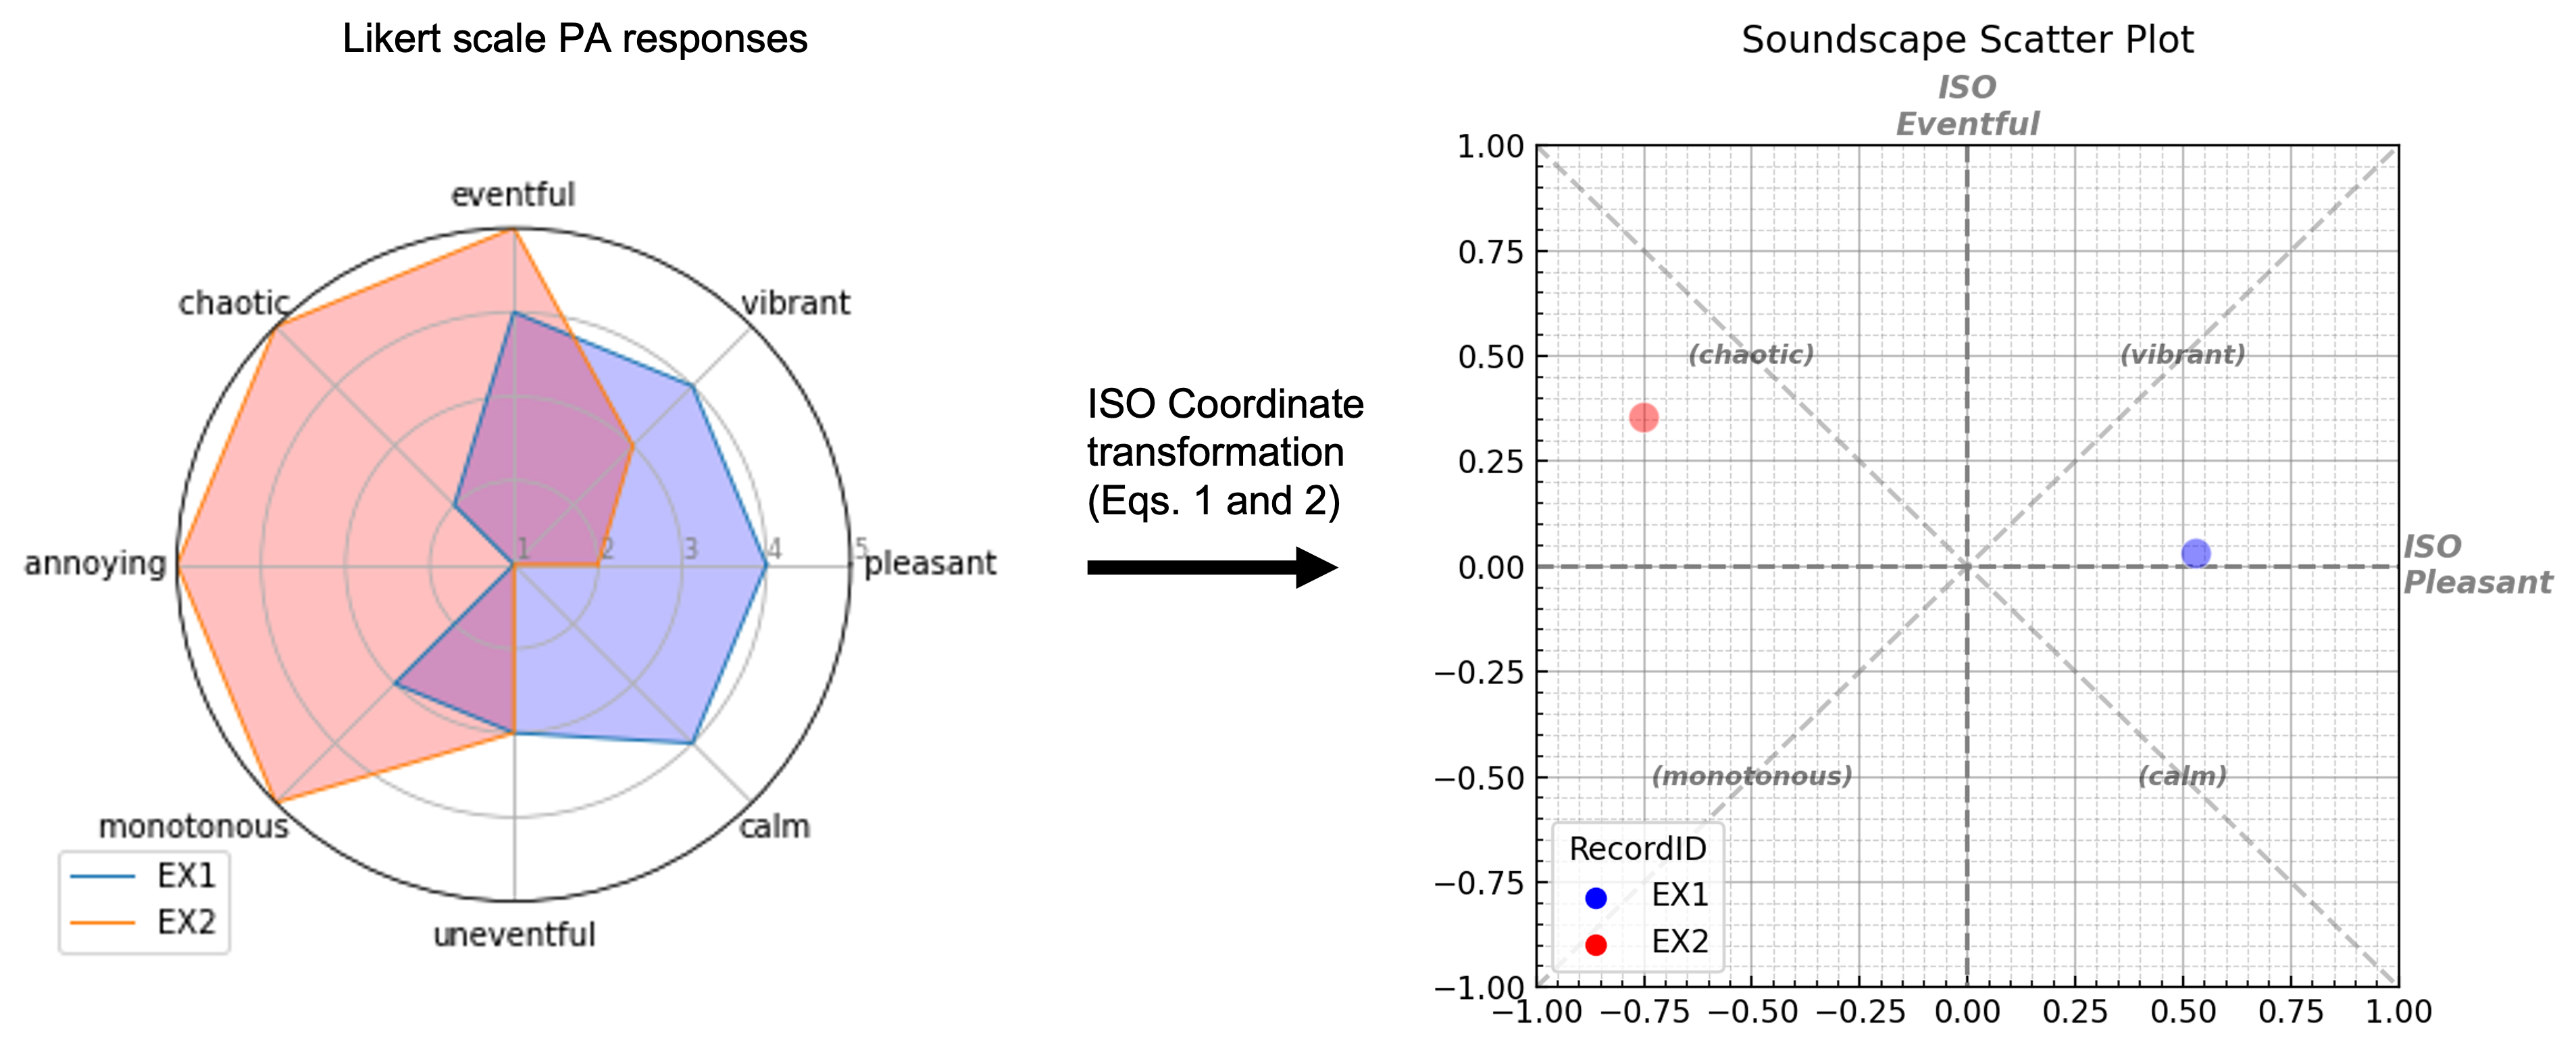
\includegraphics[width=\textwidth]{Figures/jasa-el_Figure1.png}
  \caption{Example of representations of two soundscape assessments. Left: Radar plot of two example perceptual attribute (PA) ratings on the Likert scales (1 to 5). Right: Scatter plot of the same assessments on the soundscape circumplex, transformed according to ISO 12913 Part 3.
    \label{fig:radar}
  }
\end{figure}

\section{Interpreting the Soundscape Circumplex}
\draft{Needs to be edited and connected to rest of chapter.}
%Move this paragraph to the interpretation of the circumplex section.
The circumplex model of soundscape, as originally defined by \citet{Axelsson2010principal}, is commonly understood to be a two-dimensional space (its main orthogonal components being annoying-pleasant and uneventful-eventful) where all regions of the space are equally likely to accommodate a given soundscape assessment \citep{Aletta2016Soundscape}. For instance, in theory, an extremely vibrant soundscape (e.g., with a score of 1) should be as likely to occur as an extremely annoying one, as well as one neutral on all dimensions (e.g., with a score of 0). However, a recent work by Lionello et al. \citep{Lionello2021Introducing} incidentally highlighted a possible issue with the process for representing soundscape assessments with the current ISO protocols. More specifically, when considering big numbers, soundscape assessments seem to have a bivariate normal distribution around the origin of the circumplex model. This would imply that not the whole space of the model is equally accessible to any given soundscape. Studies in the field show that data collection campaigns rarely return extreme values for soundscape dimensions \citep{Mancini2021Soundwalk} and so far the general interpretation has been that some soundscapes (e.g., extremely monotonous) may simply be difficult to find and detect with people in urban contexts \citep{Sun2019Classification}.

\subsection{Application \& Simulations}
In order to investigate the shape of the circumplex coordinate space generated by this transformation, a dataset of 3 million randomly simulated PA responses was generated. For each of the 8 PAs, an integer value from 1 to 5 is randomly generated from a uniform distribution, meaning each of the five responses is equally likely. These simulated data are specifically not intended to include any information about correlations between the various PAs when actually answered by respondents (see \citep{Lionello2021Introducing} for more on this discussion), instead the PA responses are completely uncorrelated as they each have their own random distribution. Therefore, the simulated dataset represents a theoretical uniform coverage of the 8 dimensional PA space.

We then apply the ISO transformations given in \cref{eqn:pleasant,eqn:eventful}, resulting in 3 million coordinate pairs with a range of (-1, 1) in the x and y axes. A heatmap of the resulting two-dimensional circumplex space is shown in \cref{fig:isoheatmap}, along with histograms of the individual dimension distributions. These distributions then represent the theoretical available circumplex space generated by the ISO transformation on uniform survey responses.

\begin{figure}
  %TODO: Insert heatmap figure, with histograms/distribution plots of individual axes
  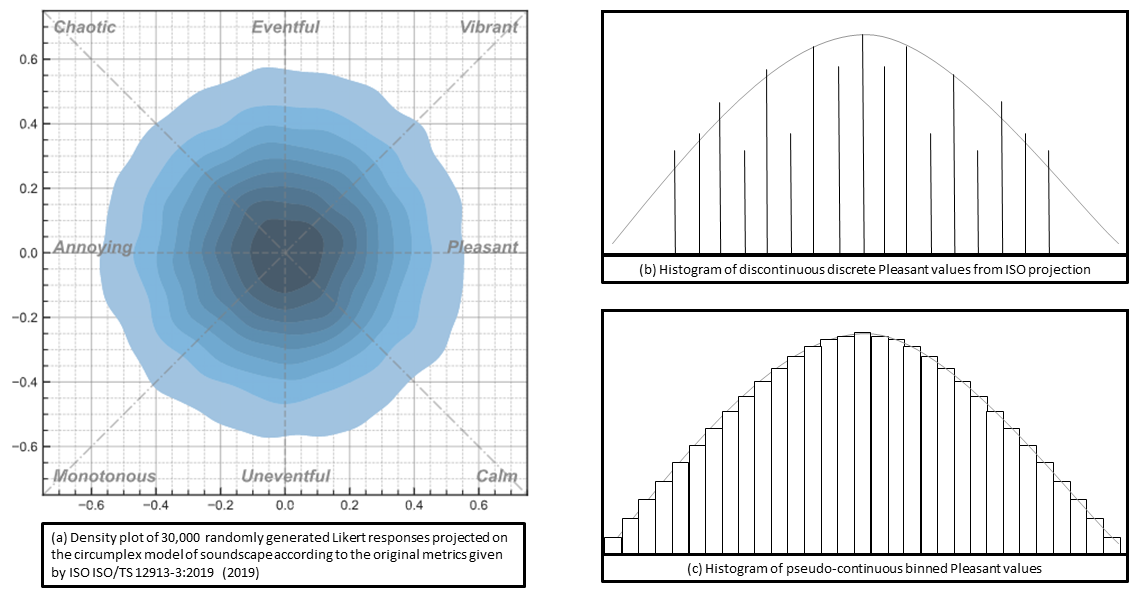
\includegraphics[width=\textwidth]{figures/Combined_sim_hist_mockup.png}
  \caption{Mockup placeholder simulation heatmap plot from Lionello 2020 and discrete vs binned transformation values. For new one, need to include distribution histograms along each axis.%
    \label{fig:isoheatmap}
  }
\end{figure}

Two important observations can be made about the shape of the resulting two-dimensional distribution. The first is that the shape of the available space is a circle. It should be noted that, despite what the term 'circumplex' may indicate, the perceptual dimensions are not necessarily intended to circumscribe a circle. The second is that, in each dimension, the responses are normally distributed, centered around zero. These points will be discussed in detail below.

\subsection{Circular space discussion}
%TODO: fill in circular discussion.
Visualisations of the circumplex model in soundscape literature tend to present it as circumscribing a circle (see Figure 1 in \citep{Axelsson2010principal} and Figure 3 in \citep{Torresin2020Indoor}), and this shape is further emphasised by the initial figure in \citet{Russell1980circumplex}'s original formulation of the concept. However, it should be emphatically noted that all of these presentations are in fact artefacts of the analysis methods which generated them, not some sort of revealed pattern in the component attributes which make up the circumplex. In \citet{Russell1980circumplex}, this first figure is generated by asking respondents to place each of the 27 attributes around a circle, according to their perceived spatial relationships - the circle shape was pre-imposed on the study. In both \citet{Axelsson2010principal} and \citet{Torresin2020Indoor}, the figures are generated via Principle Components Analysis (PCA) which, again, presents these results superimposed on a circle. It is perhaps a weakness of these two, otherwise strong and impactful, papers, that they did not recognise this consequence and challenge the circular arrangement.

If we turn back to Russell's original work on the circumplex model of affect, we can see some indications that a circle does not, in fact, describe the spatial relationship of the perceptual attributes. Fig. 4 of \citep{Russell1980circumplex}, which did not pre-impose the circular arrangement in its analysis, instead most closely resembles a square with rounded corners. Continuing from this conception, when Russell presents a graphical method of assessing the two dimensions of affect (pleasure and arousal) \citep{Russell1989Affect}, they use a square grid. This is all to say that, although the term 'circumplex' and the foundational analyses which lead to a soundscape circumplex may lead us to assume it must take the form of a circle, both the framework laid down by Russell and the common treatment of the spatial relationships of the attributes actually describe a square, instead.

This treatment of the 8 PAs makes several assumptions and inferences about the relationships between the dimensions. As stated in the standard \citep[p. 5]{ISO12913Part3}:

\begin{quote}
  According to the two-dimensional model, vibrant soundscapes are both pleasant and eventful, chaotic soundscapes are both eventful and unpleasant, monotonous soundscapes are both unpleasant and uneventful, and finally calm soundscapes are both uneventful and pleasant.
\end{quote}

From this, we would infer that a maximally vibrant soundscape is both maximally pleasant and maximally eventful. However, when the projection transformation is applied it imposes certain limitations on the relationships between the dimensions which do not conform with this assumption. As shown in \cref{fig:radar}, when a soundscape is maximally vibrant (i.e. a diagonal vector distance of 1), the maximum pleasantness value it can have is determined by the $\cos 45\degree$ term, giving a max pleasantness value of $\sim0.7071$. The implication of this is that no soundscape can be both maximally pleasant and maximally eventful at the same time, meaning that these dimensions are not in fact considered as orthogonal, and that a highly vibrant soundscape cannot be considered highly pleasant or highly eventful. Similarly, if a soundscape were to begin at a maximum Eventfulness, with neutral Pleasantness, in order for the soundscape to become more pleasant, it must by definition become less eventful. This is not conceptually correct or borne out in the treatments of previous literature. These same relationships and violations hold true for the other diagonal dimensions, chaotic, calm, and monotonous.

This implication violates both the assumptions made within the formulation of the circumplex model and the way that soundscape practitioners have understood and presented the interpretations of soundscapes within the circumplex space. In cases where the PA dimensions are referred to directly \citep{steele2016evaluation, steele2019soundtracking} and those which have made use of the Part 3 transformation to 2-dimensional coordinates \citep{Mancini2021Soundwalk, Lionello2021Introducing, Manzano2021importance}, \emph{Check Manzano2021importance} the conflation of maximal values on the diagonal axes with maximal values on the primary axes is made, as in the assumptions made by the standard. This is the first of the common understandings of the circumplex which are violated by the trigonometric transformation.

\subsection{Normal distribution discussion}
%TODO: fill in normal discussion

We can also see from the histograms included along the axes of \cref{fig:isoheatmap} that the projection creates a normal distribution in both dimensions. % TODO: edit this phrasing to match the final figure
It is important here to remember that the input to the projection formulas were uniform distributions for each of the 8 PAs, and it is the projection into the two primary dimensions which results in this normal distribution.
From the simulated distributions, we can derive a normal probability density distribution (PDF) for each of the dimensions.

\[   f_X(x) = \frac{x^{-(x-\mu)^2/(2\sigma^2)}}{\sigma \sqrt{2\pi}}\]
% ! TODO: Need to pull the actual standard deviation value.
with a mean $\mu = 0$ and standard deviation $\sigma = 0.3$.

\paragraph*{Realistic max values}
\draft{Review this}
% ! TODO: Andrew update this with the actual values from the calculations!
When looking at the distribution heatmap in \cref{fig:isoheatmap}, it is useful to picture the gradients as representing the available space in the circumplex model. The probability of reaching a given result decreases as we move farther away from the origin. This means, for example, that the probability of getting a pleasantness value between 0.2 and 0.3 is nearly 4 times the probability of getting a value between 0.5 and 0.6. This may not seem important, but the consequence is that, as a result of strictly the projection calculation, neutral values within the soundscape circumplex are much more likely and the space available to compare soundscapes within is truncated.

When we start to think about real-world urban soundscape data collection, where the discussion of the soundscape of a space is not limited to a single person's perception, we need to start thinking in statistical terms. Theoretically, the limits of the projected Pleasantness are (-1, +1), however according to the PDF calculated above less than 10\% of values fall outside the range (-0.5, +0.5).
% Note: Maybe this should be moved to Proposals or Discussion section?
It may be argued that as long as +1 can theoretically be reached, this should be what is considered the maximum value for that dimension. However, in any situation which involves using multiple individual soundscape assessments in order to characterize the overall soundscape of a location, this max will effectively never be reached. According to the large-scale, multi-location data set reported in our previous study, it appears that the effective maximum values for Pleasantness and Eventfulness for the combined assessment of multiple people for a space is in reality approximately (-0.6, +0.6) \citep{Lionello2021Introducing}.

As such, extreme values on each of the perceptual dimensions are less likely to occur than are coordinate values which place the soundscape in the neutral areas of the circumplex space. This means an extremely calm (or chaotic, or vibrant, or pleasant) coordinate is significantly less likely to occur than a neutral coordinate.


\subsection{Non-continuous projected values}
\draft{May want to remove this}
% Very brief presentation of this potential issue
An implicit assumption of the transformation is that the resulting coordinates are now continuous values, which allows linear regression and correlation methods to be used. Indeed, the transformation of the 8-dimensional ordinal Likert scale data to the two-dimensional coordinates creates a higher resolution of intervals, which would appear to be pseudo-continuous. Upon further investigation, the transformation actually results in XX discrete possible values. \cref{fig:isoheatmap}(b) shows a histogram of this raw output from the transformation, demonstrating that these discrete values, while following the general normal distribution discussed above, are not evenly filled - some adjacent values may be much more or less likely than their neighbours. This poses potential issues for further analysis which assumes either continuous or equally-spaced discrete values.



 \subsection{Likert Responses}

 \subsection{Circumplex Projection}

\section{Psychoacoustics and Auditory Perception}

 \subsection{Psychoacoustic Parameters}

   \subsubsection{Loudness}
   \emph{Zwicker and Fastl, Chap 8, see Mendeley notes and python-acoustics development notes.}

\section{Machine Learning and Regression Techniques}
Machine learning approaches are typically divided into three broad categories: supervised, unsupervised, and reinforcement learning. In supervised learning, the training data consists of input-output pairs and learns a model which can map from the inputs to the outputs. In unsupervised learning, no corresponding output data is available to the training model, thus it learns patterns in the input without feedback. Reinforcement learning does not necessarily begin with training data, instead the learning agent is given a series of reinforcements in the form of rewards and punishments \citep{StuartRussell2021}. Reinforcement learning will not be used in this thesis. Unsupervised learning has been applied to a limited degree to the acoustic data collected in several sound environments which will be expanded upon later. 

The majority of this thesis is therefore focussed on creating a supervised learning model wherein the input data are the result of measurements and the output data are the perceptual assessments of the soundscapes. In the context of this thesis, there are two primary types of supervised machine learning models - regression and classification. Regression is applied when the output is a continuous number (e.g. temperature) whereas classification is used when the output is a finite set of values. 

As will be further expanded upon in \cref{ch:circumplex}, using the trigonometric projection method provided in \citet{ISO12913Part3} enables us to transform the 8 Likert scale PAQ values into a pair of coordinate values. This transformation has a few beneficial effects for applying standard modelling techniques to soundscape data. First, it simplifies and reduces the target problem; rather than needing to model eight separate responses, we are now focussed on only two. Second, it transforms the data from ordinal responses on a 1 to 5 scale into continuous values between -1 and +1. While it is clearly possible to model ordinal outputs through classification, the methods are often less familiar and more complicated than dealing with a more standard regression problem. For those outside of machine learning (i.e. designers, engineers, etc.) regression methods, especially linear regression, are already familiar and interpretable while methods of classification and ordinal modelling are typically less familiar. By applying the \gls{iso} projection to each individual's soundscape assessment, we generate a vector of output values which can be matched up to physical data measured for each individual. This creates the sort of input-output pair vector necessary for supervised regression learning.

\subsection{Multi-level Linear Regression}

Multi-level regression modelling is a technique commonly used in fields such as psychology \cit{42, 43 from Orga paper}, and \draft{other examples}. \glspl{mlm} are particularly useful when data is organised at one or more levels or groups. The concept behind \glspl{mlm} can be built up starting from simple linear regression, as given by:

\begin{equation}
  y_i = X_i\beta + \epsilon_i
\end{equation}

For a classical multiple linear regression, we expand the $k$ coefficients out as so:

\begin{equation}
  y_i = \beta_i X_{i1} + \ldots + \beta_k X_{ik} + \epsilon_i \text{ for } i = 1, \ldots, n,
\end{equation}

where the errors $\epsilon_i$ have independent normal distributions with mean 0 and standard deviation $\sigma$

Their primary feature is the ability to have coefficients and intercepts which are allowed to vary depending on the group \citep{Gelman2006Multilevel}. This can take three forms:

\begin{enumerate}
  \item Random intercepts
  \item Random slopes
  \item Random intercept and random slopes
\end{enumerate}

In a random intercept structure, the intercept for each input feature is allowed to vary according to the second level. This structure assumes that the linear relationship between each input feature and the output is consistent across the second level groups, but that the zero point (the intercept) is different. This is expressed mathematically as:

\begin{equation}
  %TODO: insert random intercept equation from Gelman 2006.
\end{equation}

In the context of auditory perception studies, this is most appropriate for repeated measures experimental designs (as will be demonstrated in \cref{ch:whostudy,ch:mlmann}). A repeated measures study is one in all participants experience all levels of the independent variables and provide some response in terms of the output variable. In other words, each participant constitutes a group in the model and they respond to all of the input variables \citep{Kristjansson2007Multilevel}. In this case, the \gls{mlm} framework is used to account for starting differences between respondents; populations are expected to demonstrate similar behaviours in response to a given stimulus, but may have differing initial starting points, i.e. different intercepts for each analysed feature. The \gls{mlm} framework using a varying intercept for each participant allows this initial difference among individuals to be accounted for while also highlighting the overall relationship between e.g. acoustic features and annoyance ratings for a given sound. 

Random slope structures take the opposite assumption; each level shares the same intercept, while the coefficients for each feature are allowed to vary depending on the group. This assumes that different groups will have a different relationship between the input features and the output, but that these relationships may begin at a different threshold. This structure appears to be less commonly used than random intercept models. This can be mathematically described as:

\begin{equation}
  %TODO: insert random slope equation from Gelman 2006
\end{equation}



The structure inherent within the \gls{isd} means that this approach is particularly appropriate. In order to further demonstrate the structure and use of an \gls{mlm}, I'll further describe it in terms of the \gls{isd} data, where the most obvious second level for this \gls{mlm} is the location (a categorical variable defined by the LocationID). 

%TODO: Finish mlm section

\paragraph*{Repeated Measures}


 \subsection{Feature Selection}
  %  \subsubsection{Mutual Information}
  %  \draft{It appears that mutual information is related to the Bayes formula. I still need to read more into this, but it appears based on relative and overlapping probability distributions between the variables in question.}
  %  \paragraph*{From scholarpedia:}
  %  % http://www.scholarpedia.org/article/Mutual_information
  %  \draft{Based on entropy, where the uncertainty about a variable can be expressed as "the number of yes/no questions it takes to guess a random variable, given knowledge of the underlying distribution and taking the optimal question-asking strategy". "The mutual information is therefore the \emph{reduction} in uncertainty about variable $X$, or the expected reduction in the number of yes/no questions needed to guess $X$ after observing $Y$.". }

  %  \draft{"Mutual Information is just one way among many of measuring how related two variables are. However, it is a measure ideally suited for analyzing communication channels. Abstractly, a communication channel can be visualized as a transmission medium which receives an input $x$ and produces an output $y$. If the channel is \emph{noiseless}, the output will be equal to the input. However, in general, the transmission medium is noisy and an input $x$ is converted to an output $y$ with probability $P_{Y|X}(y|x)$. }
  %  \misc{This seems very useful for my conception of sound perception / auditory processing, where the perception system is a noisy communication channel.}

  %  \subsubsection{Conditional Mutual Information}
  %  The Mutual Information between two variables, given another variable as a control.

%  \subsection{Clustering Analysis}
%    \paragraph{K-means}
%    \paragraph{nbclust}

